\documentclass[12pt]{article}
\usepackage[utf8]{inputenc}
\usepackage[T2A]{fontenc}
\textheight = 23cm
\textwidth = 16cm
\oddsidemargin = 5mm
\evensidemargin = -5mm
\topmargin = -2.5cm
\parindent = 24pt
\tolerance 3000
\linespread{1.5}
\usepackage[russian]{babel}
\usepackage{mathrsfs}
\usepackage{amssymb}
\usepackage{amsmath}
\usepackage{paracol}
\usepackage{comment}
\usepackage[left=2.5cm,right=2cm,
top=2cm,bottom=2cm,bindingoffset=0cm]{geometry}
\usepackage{listings}
\usepackage[dvips]{graphicx}
\usepackage[usenames]{color}
\usepackage{colortbl}
\graphicspath{{figures/}}
\usepackage{caption}
\usepackage{lipsum}
\usepackage{titlesec}
\titlelabel{\thetitle.\quad}
\newcommand\round[1]{\left[#1\right]}

\setcounter{tocdepth}{5}

\begin{document}
	\titlepage
	\begin{figure}
		\begin{center}
			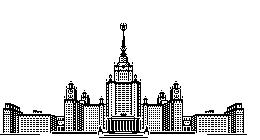
\includegraphics[width=200pt]{msu.jpg}
		\end{center}
	\end{figure}
	
	\centerline{Московский Государственный Универститет им. М. В. Ломоносова}
	\centerline{Факультет Вычислительной Математики и Кибернетики.}
	\centerline{Кафедра информационной безопасности.}
	\vfill
	\Large
	\centerline{Садовников Алексей Андреевич}
	\vfill
	\normalsize
	\centerline{\bf \LARGE Исследование существующих атак}
	\centerline{\bf \LARGE на видеопоследовательности}
	\vfill
	\Large
	\centerline{Курсовая работа}
	\vfill
	\normalsize
	\rightline{\bf Научный руководитель:}
	\rightline{Ильюшин Евгений Альбинович}
	\vfill
	\centerline{Москва, 2021}
	\clearpage
	
	\tableofcontents 
	\newpage
	
	\section{Введение}
	    $\qquad$Широкое распространение недорогих и портативных устройств видеозахвата, таких как цифровые камеры и мобильные телефоны, в сочетании с заметным ростом использования камер наблюдения, привело к внезапному увеличению объема цифровых аудиовизуальных данных, которые генерируется каждый день. А также технологические достижения различных инструментов для редактирования видео и изображений достигли такого уровня, что подделка цифрового видео или изображения может быть легко осуществима без ухудшения их качества и без каких-либо визуальных доказательств. В последние года особенно сильно возросло количество поддельных видео. Видео и изображения, доступные на различных платформах социальных сетей, таких как VK, YouTube, Facebook и др. играют жизненно важную роль в научном развитии и социально-экономическом восприятии. Помимо этого, видео используются в различных приложениях, таких как юридические доказательства, видеоуроки, реклама, видеонаблюдение. Злоупотребление или распространение неверной информации может производится через видео, т.е видео для широкого просмотра, например на YouTube или на каких-то телевизонных телеканалах может быть подвергнуто фальфикации. 
	    \newline
	    \centerline{Пример подделки видео}
	    \begin{figure}[h!]
	        \centering
	        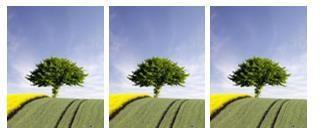
\includegraphics[width = 210 pt]{1.jpg}
	        \caption{На картинке есть дерево}
	    \end{figure}
	    \begin{figure}[h!]
	        \centering
	        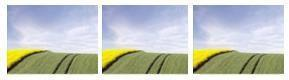
\includegraphics[width = 200 pt]{2.jpg}
	        \caption{На картинке дерево было удалено}
	    \end{figure}
	   \newline
	   $\qquad$Была произведена атака удаления объекта в исходной последовательности видеокадров и на второй картинке уже нет дерева. Если видеть кусок данной видеопоследовательности впервые, то уличить визуально в подделке довольно сложно. 
	   
    \section{Цель работы}
        $\qquad$Исследовать существующие атаки на видеопоследовательности и некоторые методы их обнаружения.
        \newline
        Для достижения поставленной цели необходимо решить следующие задачи:
        \begin{enumerate}
            \item Исследовать какие существуют виды атак на видеопоследовательности.
            \item Проанализировать методы обнаружения атак на видеопоследовательности.
       \end{enumerate}
    \newpage
    \section {Атаки на видеопоследовательности}
         $\qquad$Непрерывная видеопоследовательность - $V(x,y,t)$ скалярная функция координат $x$, $y$ и времени $t$. $B(x,y,t)$ - вектор модификации. $M(x,y,t)$ - подделанное видео, которая определяется как: $M(x,y,t) = B(x,y,t) + V (x,y,t)$. Когда содержание информации, создаваемой данной видеопоследовательностью, злонамеренно изменяется, это называется подделкой видеоданных. Видеопоследовательность можно рассматривать как набор последовательных кадров с временной зависимостью в трехмерной плоскости. 
    \subsection {Классификация атак}
        $\qquad$Есть несколько возможных атак, которые могут быть применены для изменения содержимого видеоданных. Вмешательство в видео может либо изменить его содержимое, либо повлиять на временную зависимость между кадрами.
        \newline
        \newline
        \centerline{}
        \begin{figure}[h!]
            \centering
            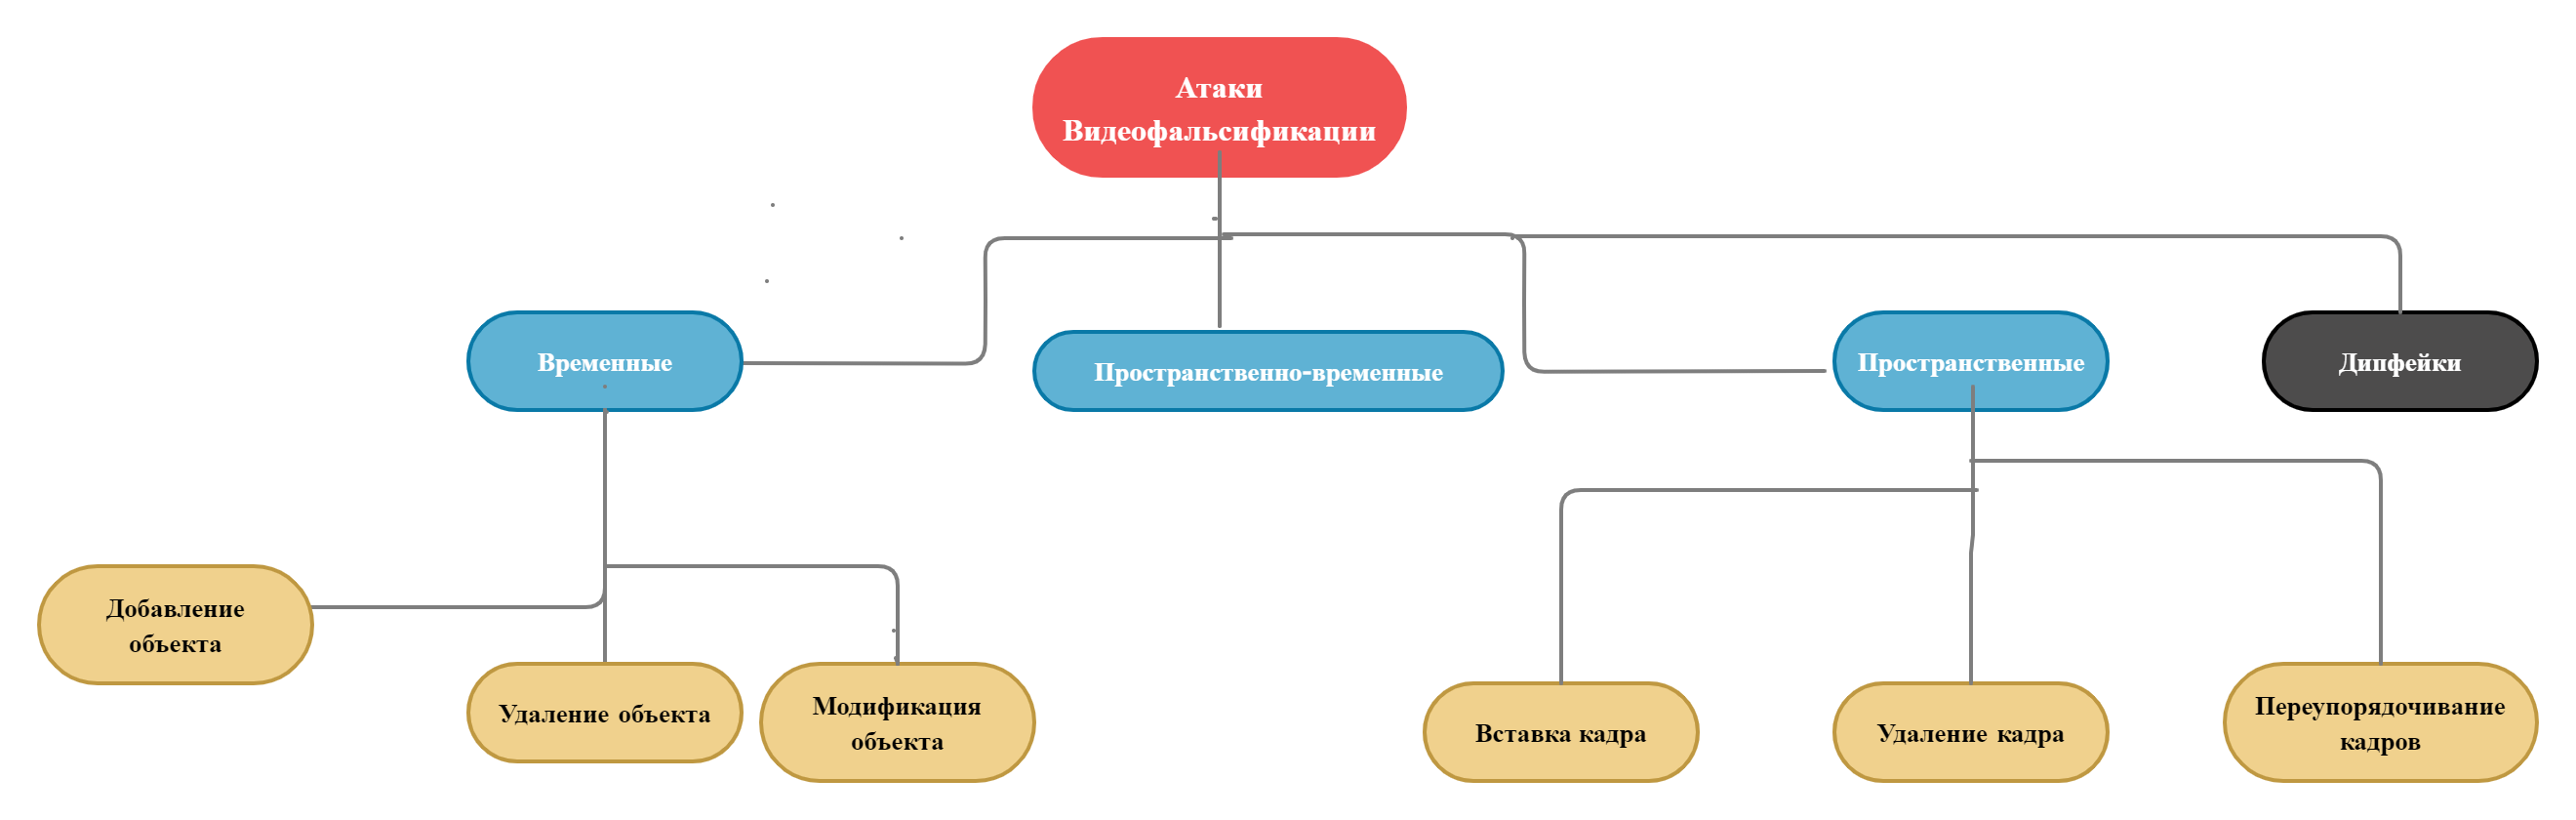
\includegraphics[width = 530 pt] {3_2.jpg}
            \caption{Схема классификации}
        \end{figure}
        \newline
        $\qquad$Атаки видеофальсификации разделяют на три основных области и еще одну отдельную дополнительную: 
        1) пространственная фальсификация
        2) пространственно-временная фальсификация
        3) временная фальсификация 
        4) дипфейки
        
    \newpage
    \subsection{Пространственное вмешательство}
        $\qquad$При пространственном редактировании вредоносные модификации изменяют содержимое одного или нескольких кадров.
        \newline
        \begin{figure}[h!]
            \centering
            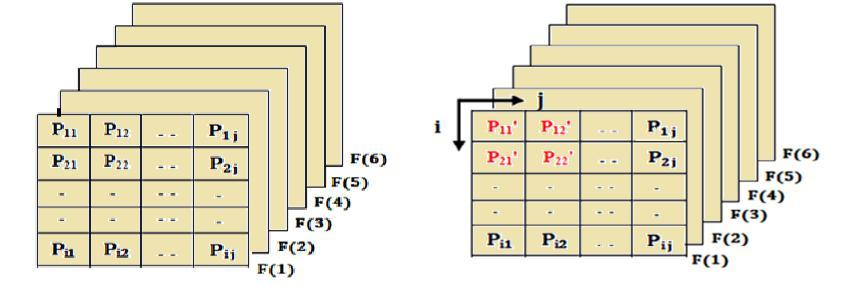
\includegraphics {4.jpg}
            \caption{Пространственное вмешательств}
        \end{figure}
        \newline
        $\qquad$Внутрикадровое вмешательство показано на Рис. 4, на котором в кадре F(1) исходного входного видео $V_0$ пространственны искажены пиксели в левом верхнем углу матрицы для создания поддельного видео $V_t$. (i,j) обозначают высоту и ширину кадров входного видео соответственно.
        \newline
        Cодержимое видеокадров обрабатывается как объекты. Объекты кадров можно разделить на два условных класса: объекты переднего плана и заднего плана. 
        \newline
        Объекты переднего плана – это те, которые фиксируются как отдельные элементы в кадре без фона. 
        \newline
        Фоновый объект – это фоновая часть часть кадра, за исключением всех объектов переднего плана.Атаки такого типа могут быть эффективно выполнены с помощью программного обеспечения для редактирования видео, например с помощью Adobe After Effects. К различным типам атак пространственного вмешательства относятся добавление объекта, удаление объекта и модификация объекта. 
    \subsubsection {Атака с добавлением объекта}
        $\qquad$Эта атака может выполняться с объектами обоих типов, объектами заднего плана и объектами переднего плана. Копия-подделка с перемещением или подделка с копированием и вставкой является примером атаки с добавлением объектов. Используя эту атаку, злоумышленник может вставить или удалить объект в сцене, изображенную на видеокадрах. 
        \newline
        \begin{figure}[h!]
            \centering
            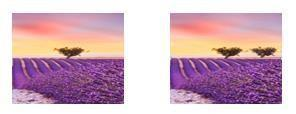
\includegraphics {5.jpg}
            \caption{Атака с добавлением объекта}
        \end{figure}
        \newline
        На картинке показан пример подделки «копирование-перемещение», в котором дополнительное дерево в качестве объекта переднего плана копируется из исходного кадра и добавляется в другое место в том же кадре.
    \subsubsection{Атака с удалением объекта}
         $\qquad$В такой атаке удаляются объекты на кадрах видео. Эта атака может выполняться как с фоновым объектом, так и с объектом переднего плана. Для восстановления удаленных или поврежденных областей визуально правдоподобно можно использовать метод «рисование». Его можно использовать обычно двумя способами. Либо удаленные области заполняются с помощью образцов текстур, либо наиболее взаимосвязанные блоки из смежных по времени кадров используются для заполнения удаленной области. Еще есть подвид атаки - высококвалифицированная обрезка, при которой кадры видео обрезаются, чтобы удалить доказательства совершения подмены видео, а затем увеличивают поврежденные кадры, чтобы сохранить постоянное разрешение по всему видео. 
        \newline
        \begin{figure}[h!]
            \centering
            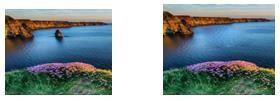
\includegraphics {6.jpg}
            \caption{Атака с удалением объекта}
        \end{figure}
        \newline
         На картинке показан пример атаки удаления объекта, при которой объект переднего плана удаляется из исходного видеокадра.
    \subsubsection{Атака с модификацией объекта}
        $\qquad$При атаке модификации объекта существующий объект кадра может быть изменен таким образом, что первоначальная идентичность этого объекта теряется. Эта атака может быть выполнена как с фоновыми, так и с передними объектами. Возможны изменения размера, формы объекта, цвета объекта, а также с помощью дополнительных эффектов изменение характеристики объектов и его связь с другими объектами. Эти атаки выполняются на уровне пикселей. Эта атака считается довольно сложной для обнаружения. Фактически,  DeepFakes - частный случай этой атаки.
        \newline
        \begin{figure}[h!]
            \centering
            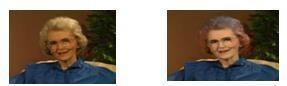
\includegraphics[width = 200 pt] {7.jpg}
            \caption{Атака с модификацией объекта}
        \end{figure}
        \newline
    \subsection{Временное вмешательство}
        $\qquad$Временная фальсификация видео – тип вмешательства, применяемый к видеокадрам, влияющий на временную последовательность визуального контента.Основное внимание уделяется временной
        зависимости. К распространенным атакам этого типа относят: вставку кадра, удаление кадра, переупорядочивание или перестановка кадров.
        \newline
        \begin{figure}[h!]
            \centering
            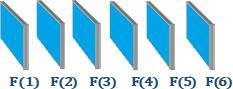
\includegraphics[width = 180 pt] {8.jpg}
            \caption{Последовательность 6 кадров в исходном видео $V_0$}
        \end{figure}
        \newline
    \subsubsection{Атака с вставкой кадра}
        $\qquad$При этой атаке вставляются дополнительные кадры из другого видео, которое имеет те же статистические свойства,кадры намеренно вставляются в некоторые произвольные места в данном видео. При этом счетчик кадров увеличивается при вставлении новых кадров в исходное видео. Основная цель такой атаки – замаскировать исходный контент и предоставить ошибочную информацию. 
        \newline
        \begin{figure}[h!]
            \centering
            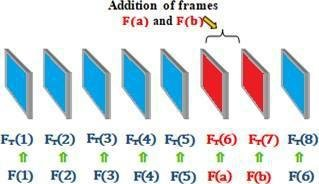
\includegraphics[width = 220 pt] {9.jpg}
            \caption{Атака с вставкой кадра}
        \end{figure}
        \newline
        На картинке пример, в котором два квадра F(a) и F(b) вставлены в случайном месте в исходное видео для создания искаженного видео, состоящего из восьми кадров.
    \subsubsection{Атака с удалением кадра}
        $\qquad$При атаке с удалением кадра, кадры удаляется намеренно из разных мест или могут быть удалены из определенного места. Количество кадров уменьшается, когда кадры удаляются из исходного видео. В зависимости от мотива это обычно выполняется при видеонаблюдении, когда злоумышленник хочет убрать свое присутствие на видео. 
        \newline
        \begin{figure}[h!]
            \centering
            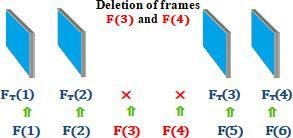
\includegraphics[width = 210 pt] {10.jpg}
            \caption{Атака с удалением кадра}
        \end{figure}
        \newline
        На картинке показан типичный пример атаки с удалением кадра из видеопоследовательности длиной 6 кадров, при котором кадры, помеченные F(3) и F(4) удаляются из исходного видео для создания поддельного видео, состоящего всего из четырех кадров.
    \subsubsection{Атака с перестановкой кадров}
        $\qquad$При этой атаке кадры переупорядочиваются или перемешиваются таким образом, что фактическая последовательность видеокадров перемешивается и видео генерирует ошибочную информацию по сравнению с исходным видео. При этом счетчик кадров остается неизменным.
        \newline
        \begin{figure}[h!]
            \centering
            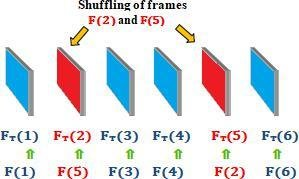
\includegraphics[width = 210 pt] {11.jpg}
            \caption{Атака с перестановкой кадров}
        \end{figure}
        \newline
        Типичный пример атаки с переупорядочиванием кадров, в которой 2 и 5 кадр меняются местами.
    \subsection{Пространственно-временная фальсификация видео}
        $\qquad$Пространственно-временная фальсификация видео - сочетание пространственного и временного вмешательства, можно найти как межкадровые, так и внутренние подделки. Система аутентификации должна быть достаточно надежной, чтобы распознать оба вида взлома.
        \newpage
        \begin{figure}[h!]
            \centering
            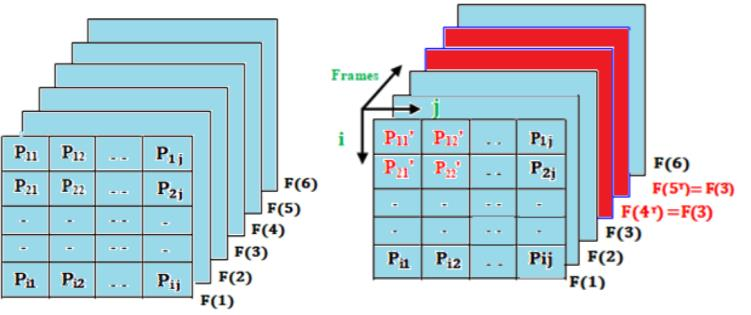
\includegraphics[width = 220 pt] {12.jpg}
            \caption{Пространственно-временное вмешательство}
        \end{figure}
        i,j обозначают высоту и ширину входной последовательности видеокадров. Видно, что в результате временного вмешательства были переставлены кадры: а именно в результате временного вмешательства на место 4 и 5 кадров поставлен 3-ий кадр и в результате пространственного вмешательства в 1-ом кадре были изменены пиксели в левом верхнем углу матрицы пикселей.
    \subsection{Вмешательство в видеопоследовательности по уровням}
        $\qquad$Вмешательство в видео различают по уровням: на уровне пикселей, на уровне блока, на уровне кадра.
        \newline
        1)      Подделка на уровне пикселей. Наименьший уровень, на котором может быть вмешательство в видеопоследовательность. Многие обычные операции обработки видео выполняются на уровне пикселей. Система аутентификации видео должна быть достаточно надежной, чтобы различать фальсификацию на уровне пикселей и нормальное обработку видео. На уровне пикселей обычно выполняется пространственное вмешательство
        \newline
        2)      Подделка на уровне блоков. Указанная конкретная область в кадре видео называется блоком. Содержимое видеокадра рассматривается как множество блоков, над которыми выполняются вмешательства, блоки могут быть преобразованы, обрезаны, модифицированы или заменены. На уровне блоков обычно выполняется пространственное вмешательство.
        \newline
        3)      Подделка на уровне кадра. Это вставка кадра, удаление кадра, перестановка кадров – распространенные атаки взлома видеопоследовательности. На уровне кадра обычно выполняется временное вмешательство.
    \section{Методы обнаружения атак на видеопоследовательности}
        $\qquad$Методы обнаружения подделки видео можно разделить на две основные категории: активные методы обнаружения подделки видео и методы пассивного обнаружения подделки видео.
        \newline
    \subsection{Активные методы обнаружения}
        $\qquad$Активный метод обнаружения подделки видео использует предварительно встроенные скрытые данные, такие как цифровая подпись или водяной знак, для проверки подлинности и целостности цифровых видео.
        
        
    \subsubsection{Недостатки активного метода обнаружения}
        $\qquad$У активного подхода есть недостатки:
        \begin{enumerate}
            \item На этапе сбора данных требуется специальное оборудование, такое как оборудованные камеры для вставки водяных знаков или цифровой подписи в видео.
            \item  Многочисленные методы шифрования могут предотвратить несанкционированный доступ и манипулирование содержанием видео, тем не менее, эти методы шифрования не могут помешать владельцу цифрового видео
            \item Такие факторы как сжатие, масштабирование, шум и т.д влияют в худшую сторону по надежности водяных знаков и цифровых подписей.
        \end{enumerate}
    \subsubsection{Цифровая подпись}
        $\qquad$В 1976 году Диффи и Хеллман ввели цифровую подпись для аутентификации мультимедийных данных и проверки их целостности. Цифровые подписи могут быть сохранены двумя разными способами для целей аутентификации. Либо его можно сохранить как независимый файл, либо в поле заголовка сжатой исходной информации. Это оказывается лучше, потому что цифровая подпись остается неизменной даже при изменении значений пикселей изображений или видео, и это дает лучшие результаты. При такой аутентификации, цифровая подпись не может быть подделана, поскольку цифровая подпись подписывающего лица зависит от содержания данных и от некоторой секретной информации, которая известна только подписывающей стороне.
    \subsubsection{Интеллектуальные методы аутентификации}
        $\qquad$Интеллектуальные методы используют базу данных видеоклипов для аутентификации видео. База данных состоит как из подделанных, так и из подлинных видео. Основное преимущество интеллектуальной техники перед другими методами, такими как цифровая подпись и водяной знак, состоит в том, что она не требует какой-либо процедуры внедрения водяного знака или вычисления и хранения какого-либо секретного или открытого ключа.
        \newline
        Вычисляется информация о локальной относительной корреляции и классифицирует видео как поддельное или не поддельное видео. Используются алгоритмы машинного обучения - метод опорных векторов.
        \newline
        Алгоритм выполняется в два этапа:
        \newline
        1)      Этап обучения
        \newline
        2)      Этап обнаружения и классификации подделки
        \newline
        На этапе обучения алгоритм использует обучающие датасеты, помеченных вручную. Если видео в обучающих данных фальсифицировано, то назначается метка -1, а если подлинное, то +1. Из обучающих видео относительная корреляция информация между двумя соседними кадрами видео, затем вычисляется относительная корреляционная информация RC для всех смежных кадров видео с помощью: 
        $RC = \frac{1}{m}\displaystyle\sum_{i=1}^{m} L_i $ , где $L_i $ - локальная корреляция между двумя кадрами, $ m$ - количество соответствующих угловых точек в двух кадрах.  Информация о локальной корреляции $RC$ вычисляется для каждого видео и $RC$ с меткой информации обо всех обучающих видеоданных предоставляется в виде входных данных для метода опорных векторов. Со всей этой информацией обо всех видео с помощью метода опорных векторов алгоритм обучен определять является ли видео поддельным или нет.
        Концом обучения является верное построение гиперплоскости, отделяющая поддельные видео от подлинных.
    \subsubsection{Водяные знаки}
        $\qquad$Помимо проверки целостности цифровых данных и выявления злонамеренных манипуляций, водяные знаки могут использоваться для аутентификации производителя или автора контента. Водяные знаки могут быть встроены в видео, не изменяя фактического значения содержания данных. Полезная особенность водяных знаков заключается в том, что их можно встраивать без значительного ухудшения качества видео. Поскольку водяные знаки встроены в содержимое видеоданных, после изменения данных эти водяные знаки также будут изменены, это поможет использовать водяные знаки для проверки целостности мультимедийных данных. Техника нанесения водяных знаков на видео делится на два сегмента:
        \newline
        \begin{enumerate}
            \item Встраивание или кодирование водяного знака во входное видео
            Процесс нанесения водяных знаков или кодирования видео выполняется на стороне источника. В этом процессе водяной знак встраивается во входное видео с использованием любого алгоритма водяных знаков. Весь процесс можно рассматривать как функцию $V_w = E(V_i_n,W,K)$, которая сопоставляет входное видео $V_i_n$, водяной знак $W$ и ключ $K$ для вывода видео с водяными знаками $V_w$
            \begin{figure}[h!]
            \centering
            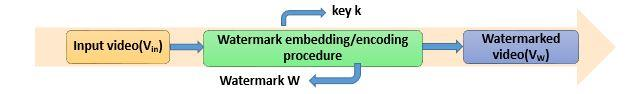
\includegraphics[width = 300 pt] {13.jpg}
            \caption{Схема: встраивание водяного знака}
        \end{figure}
            \item  Извлечение или декодирование водяного знака из видео.
        Процесс декодирования или извлечения водяных знаков из видео с водяными знаками является процессом, обратным алгоритму встраивания $V_i_n = D(V_W,W,K)$
            \begin{figure}[h!]
            \centering
            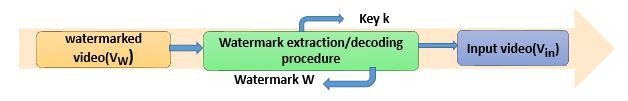
\includegraphics[width = 300 pt] {14.jpg}
            \caption{Схема: извлечение водяного знака}
        \end{figure}
        \end{enumerate}
        \newpage
    \subsubsection{Другие методы аутентификации}
        $\qquad$Помимо цифровой подписи, водяных знаков и интеллектуальных методов есть и иные способы аутентификации подделки видео. Одним из таких способов, является схема аутентификации для цифрового видео, основанная на траектории движения и совместном использовании криптографического секрета.В этой схеме видео сначала сегментируется на кадры,
        затем все кадры видеопоследовательности отображаются на траекторию в
        пространстве признаков, по которой вычисляются ключевые
        кадры видео. После того, как ключевые кадры вычислены,
        секретный кадр вычисляется на основе информации о ключевых
        кадрах видеопоследовательности. Эти секретные кадры используются для
        построения иерархической структуры, после чего получается
        окончательный главный ключ. Этот мастер-ключ используется
        для определения подлинности видео. Любые изменения в кадре
        или в важном содержании кадра будут отражены как изменения
        в вычисленном главном ключе. Траектория строится по гистограмме кадров. Как только ключевые кадры вычислены, они используются для вычисления секретного кадра путем экстраполяции.
        Интерполяционный полином $f(x)$ вычисляется с использованием ключа кадра.
        $\displaystyle\sum_{j=1}^{n+1}\displaystyle\prod_{i=1}^{n+1}\frac{x-x_i}{x_j-x_i}I_j $
        - интерполяционная формула Лагранжа, где $x_i$ - позиция относится к каждому ключевому кадру, а $I_i$ - значение пикселя ключевых кадров. Используя это уравнение и экстраполяцию, а кадр при $x=0$, считается секретным ключом. С помощью этой схемы любое видео может быть аутентифицировано путем
        сравнения его вычисленного мастер-ключа с исходным
        мастер-ключом. Это сравнение может быть выполнено с помощью
        общей меры косинусной корреляции, заданной $sim = \frac{I_0 I_N}{|I_0 I_N|}$, где $I_0$ - исходный главный ключ и $I_N$ - новый главный ключ, рассматриваемые как векторы. Значения сходства будет находиться в диапазоне $[0,1]$. Если $sim = 1$, то два главных ключа одинаковые, а если $sim = 0$, то два главных ключа полностью разные.
    \subsection{Пассивные методы обнаружения}
        $\qquad$Иное название пассивных методов - методы слепого обнаружения. Эти методы, которые можно использовать для проверки подлинности видео вне зависимости от предварительно встроенных или предварительно извлеченных данных. Обнаружение пассивного вмешательства включают обнаружение редактирования на основе камеры, на основе артефактов кодирования, на основе несоответствий в содержании, обнаружения копирования-перемещения в видео.
    \subsubsection{Преимущества пассивного подхода}
        \newline
        \begin{enumerate}
            \item Для обнаружения редактирования не требуется предварительно встроенной информации в видео, она зависит только от доступного измененного видео и его внутренних функций.
            \item Для обнаружения редактирования видео не требуется специального оборудования.
        \end{enumerate}
    \subsubsection{Обнаружения редактирования пассивными методами}
        \begin{itemize}
            \item Обнаружение редактирования видео на основе камеры.
            \newline На записанных видеороликах видеокамеры оставляют характерный отпечаток пальца. Этот отпечаток пальца используется не только для идентификации устройства, но также может использоваться для обнаружения подделки видео. Прямое применение метода снятия отпечатков пальцев (неоднорость фотоответа) , в котором используются шумовые характеристики устройства сбора данных для обнаружения подозрительных областей на видео, записанном со статической сцены позволяют обнаружить подделку.
            \item Обнаружение на основе артефактов кодирования. 
            \newline На производительность метода обнаружения подделки видео в значительной степени влияет процесс кодирования видео. Кодирование видео выполняется для внедрения в видео артефактов, которые можно использовать для определения целостности видеоконтента путем его извлечения и проверки. В последние годы криминалисты в области видеонаблюдения полагаются на эти артефакты, чтобы определить целостность видео и найти в нем поврежденные области.
            \item Обнаружение несоответствий по содержанию. 
            \newline В конкретном видео сложно покадрово определить, являются ли геометрические, физические или световые свойства сцены настоящими и не поддельными. До сих пор были предложены два подхода для определения этого типа фальсификации:
            \newline
            1) подход, основанный на артефактах, которые остаются в результате рисования видео
            \newline
            2) подход, который раскрывает несоответствия в движении объектов
            \item Обнаружение копирования-перемещения в видео.
            \newline Атаки подделки копирования-перемещения может быть выполнена на видео и разделена на два этапа, которые включают подделку перемещения внутрикадрового копирования и подделку перемещения межкадрового копирования. При внутрикадровой подделке часть кадра копируется и вставляется в другом месте этого кадра. Обычно это делается для того, чтобы скрыть или дублировать какой-либо объект одного кадра или нескольких кадров. При межкадровой подделке злонамеренные модификации применяются к последовательности кадров и различные типы этой атаки включают вставку кадра, удаление кадра, переупорядочивание кадров.
     \end{itemize}
     \subsection {Общая структура обнаружения}
        $\qquad$Структура общего процесса обнаружения фальсификации видео состоит из 6 этапов.
        \newline
        Первый шаг - разделить входное видео и извлечь из него кадры. Затем следует этап «Извлечение признаков» для поиска или извлечения векторов признаков. На этом этапе используются различные методы извлечения признаков, такие как DCT (дискретное косинусное преобразование), DWT (дискретное волновое преобразование) и т.д. На следующем этапе могут быть применены методы сопоставления перекрывающихся блоков, такие как дерево K-SVD (K-сингулярное разложение) и сортировка по основанию. После выполнения сопоставления блоков выполняются операции постобработки, и на последнем решающем этапе делается вывод о типе фальсификации видео и его местонахождении в кадре.
        \begin{figure}[h!]
            \centering
            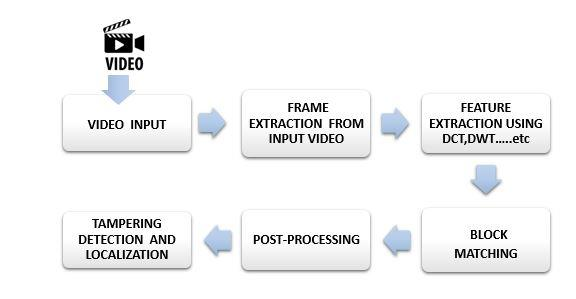
\includegraphics[width = 300 pt] {15.jpg}
            \caption{Общая схема процесса обнаружения фальсификации}
        \end{figure}
        \newline
        \newline
    \subsection{Сложные сценарии для идентификации видео}
        $\qquad$В некоторых системах наблюдения важными вопросами являются затраты на хранение и передачу данных. Для снижения затрат на хранение и передачу необходимо отправлять и хранить только те видеоклипы, которые содержат интересующие объекты. Более того, в большинстве приложений наблюдения фоновые объекты изменяются очень медленно по сравнению с объектами переднего плана. Возможное эффективное
        решение в этих сценариях заключается в том, что только объекты, представляющие
        интерес (в основном объекты переднего плана), отправляются кадр за кадром в режиме реального времени, в то время как фоновый объект отправляется один раз
        в течение длительного промежутка времени. В таких приложениях наблюдения
        становится очень важно защитить подлинность
        видео: подлинность от вредоносных изменений и
        подлинность для идентификации источника передачи (т. е.
        идентификации источника видео). В системах наблюдения, основанных на событиях, видеопоследовательность захватывается, когда происходит
        какое-либо изменение в сцене (наличие события)
        который будет запечатлен камерой. Если в сцене нет изменений, то камера наблюдения не
        захватывает никакой видеоряд. Этот вид системы наблюдения
        используется в военной системе для обеспечения безопасности границ. Аутентичность для такого рода видеопоследовательностей является
        сложной проблемой, поскольку
        в видеопоследовательностях, снятых камерой наблюдения, нет надлежащей временной последовательности.
        Это сценарии, которые создают значительные
        проблемы при проверке подлинности.
        
    \section {Дипфейки}
        $\qquad$Впервые распространение дипфейки получили в 2017 году, когда пользователь с ником "Deepfakes" на сайт Reddit начал размещать видео созданные с использованием алгоритма смены лиц на основе глубоких нейронных сетей Deep Neural Networks (DNN). Впоследствии термин DeepFake стал использоваться более широко для обозначения любых видео, в которых происходит замена лиц с помощью ИИ. Сейчас выделяют 3 основных вида видео DeepFake: 
        \begin{enumerate}
            \item Синтез видео головы и верхней части плеча нужного человека с
            исходным. Поведение сохраняется
            \item Замена лиц включает в себя создание нужное видео с лицами,
            замененными синтезированными лицами источника, сохраняя выражения лиц.
            \item Синхронизация губ. Манипулируя губами заставлять говорить то, чего
            человек на самом деле не произносил.
       \end{enumerate}
        \begin{figure}[h!]
            \centering
            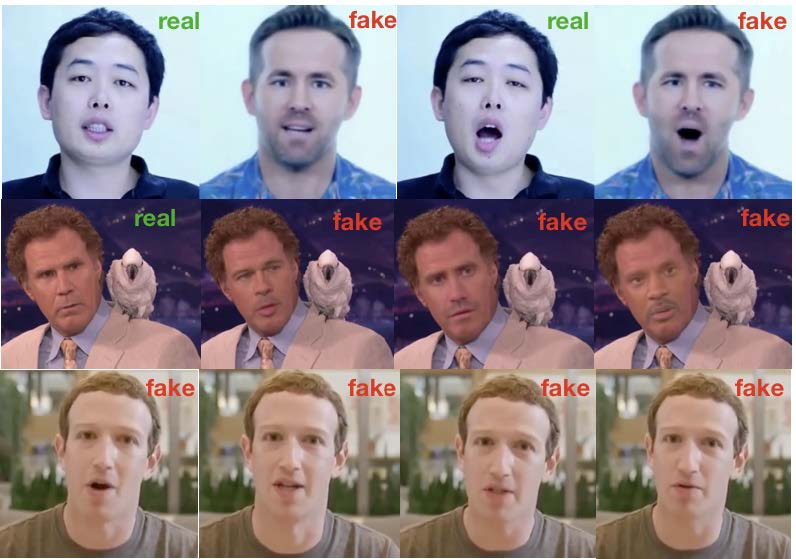
\includegraphics[width = 300 pt] {16.jpg}
            \caption{Примеры DeepFake: 1 строка - 1 вид (синтез видео головы и плечей), 2 строка - 2 вид (замена лица с сохранением выражения), 3 строка - 3 вид (синхронизация губ)}
        \end{figure}
        Хотя есть интересные и творческие применения видео DeepFake, из-за сильной ассоциации лиц с личностью человека их также можно использовать в качестве оружия. Хорошо составленные видеоролики DeepFake могут создавать иллюзии присутствия и действий человека, которые не происходят в реальности, что может привести к серьезным политическим, социальным, финансовым и юридическим последствиям.
    \subsection{Классификация методов обнаружения DeepFake}
        $\qquad$Текущие методы обнаружения DeepFake в основном нацелены на видео со сменой лиц, которые составляют большую часть видео DeepFake, распространяемых в Интернете. Многие из существующих методов сформулированы как задачи двоичной классификации на уровне кадра. В зависимости от используемых функций эти методы делятся на три основные категории, которые основаны на:
    \begin{enumerate}
        \item Физических несоответствиях. 
        \newline Во многих дипфейках отсутствует разумное моргание глаз из-за использования онлайн-портретов в качестве обучающих данных, которые обычно не закрываются по эстетическим причинам.
        \item  Артефактах. 
        \newline Визуальные артефакты видео DeepFake в существующих наборах данных, включая некачественные видимые границы сращивания, несоответствие цветов, видимые части исходного лица и несовместимые ориентации лица.
        \item Управляемых данных. 
        \newline Используют различные типы глубоких нейронных сетей, обученные на реальных видео и фейковых видео, но фиксирующие определенные артефакты.
    \end{enumerate}
    \subsection{Cдерживание увеличения количества дипфейков}
        $\qquad$Так как датасет лиц для обучения алгоритмов машинного обучения берут из сети, и очень часто используют в недобросовестных целях, то один из предлагаемых вариантов сдерживать рост количества дипфейков, собираемых в веб-пространстве - метод нарушения синтеза лиц ИИ. Метод основан на добавлении возмущения к исходному изображению, чтобы отвлечь детекторы лиц на основе DNN, так что качество полученного набора лиц в качестве обучающих данных снижается. 
         \begin{figure}[h!]
            \centering
            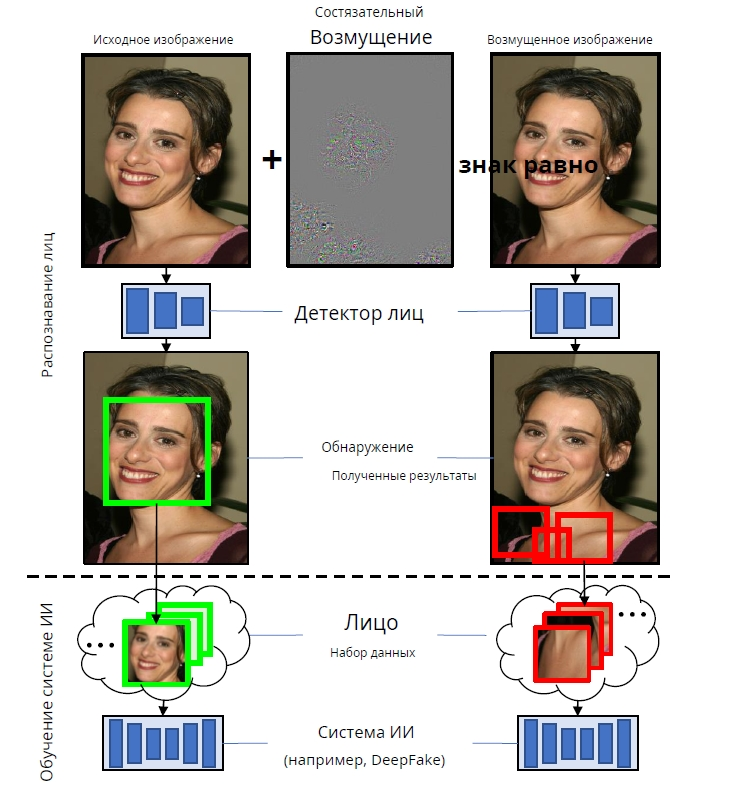
\includegraphics[width = 300 pt] {17.jpg}
            \caption{Схема метода нарушения синтеза лиц ИИ}
        \end{figure}
    \subsection{Дикие дипфейки}
        $\qquad$На данный момент в интернет выгружено достаточно большое количество дипфейков, и так как фейковая информация в этих видео потенциально создает большую информационную опасность, поэтому важно обнаруживать дипфейки. Но для обучения детекторов дипфейков требуется большой датасет из реальных и дипфейк видео. Обычные виртуальные дипфейки содержат сцены с маленьким количеством людей и похожие выражения лица, чаще всего просто разговор. А вот WildDeepFake (дикие дипфейки) сцены могут иметь огромное количество человек, более 10. А также, если обычные виртуальные дипфейки создаются с помощью популярных методов, то дикие дипфейки могут использовать различные комбинации методов и их создание более сложное. Виртуальные дипфейки чаще всего имеет низкое качество, в области лица могут быть заметные искажения, размытость и другие странные артефакты. Большинство диких дипфейков намеренно создаются в высоком качестве. В [4] был создан датасет диких дипфейков (WildDeepFake), состоящих из 707 хорошо сделанных дипфейк-видео из интернета, видеоконтент разнообразен: множество действий (например, трансляция, фильмы, интервью, беседы и многое другое), разнообразные сцены, фоны и условия освещения, а также различные степени сжатия, разрешения и форматы.
    \subsection{Генерация дипфейков}
        $\qquad$Одним из широко используемых методов глубокого обучения для генерации дипфейков являются генеративные состязательные сети (GAN). На GitHub существует множество программ для дипфейков с открытым исходным кодом, например Faceswap-GAN и Faceswap. Большинство этих программ для дипфейков используют архитектуру кодировщика-декодера с одним кодировщиком и двумя декодерами: кодировщик изучает общие черты исходного (реального) и целевого (поддельного) лица, в то время как два декодера обучаются отдельно генерировать исходное и целевое лицо. Во время процесса замены лица декодер, связанный с исходным лицом, принимает кодировку целевого лица и генерирует поддельное исходное лицо. Маска внимания исходного лица обычно используется для того, чтобы поддельное лицо источника выглядело более убедительно с помощью этапа слияния. Сгенерированные поддельные лица могут быть дополнительно улучшены за счет использования изображений лиц с более высоким разрешением (как исходных, так и целевых).
        \newline
        \begin{figure}[h!]
            \centering
            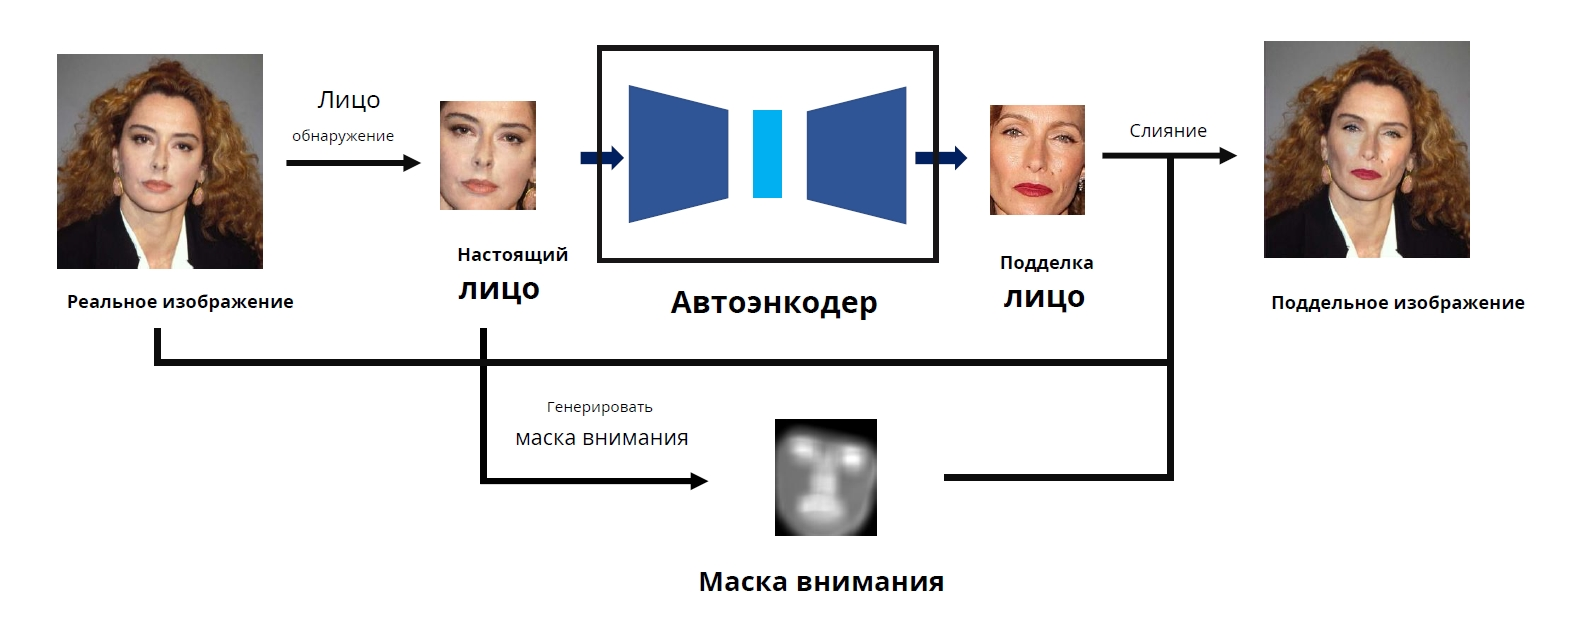
\includegraphics[width = 500 pt] {18.jpg}
            \caption{Процесс замены лиц}
        \end{figure}
        \newline
    \subsection{Сеть обнаружения Deepfake}
        $\qquad$Одной из эффективных сетей обнаружения Deepfake - сеть на основе внимания (ADDNets), которая также может достаточно эффективно определять дикие дипфейки.
        Берется набор данных $D = {(x,y)^(i)}$ где $i=1,..,n$ c $x \in X \subset R^{F*W*H*C}$ и $y \in Y = [0, 1]$ обозначающе видео и метку класса. $F,W,H,C$ - количество кадров, ширина кадра, высота кадра и цветовой канал соответственно. Два класса, $y=0$ реальные видео и $y=1$ дипфейки. Цель обнаружения дипфейка – обучить бинарный классификатор f, который отображает пространство видео в пространство классов $f: X-> Y$. Это может достигаться за счет минимизации ошибки классификации f при обучении с данных D: $\underset{\theta}{\operatorname{argmin E_(x,y)_\in_D l(f(x),y)}} $, где l-функция потерь, $\theta$ - обучаемые параметры сети.Входные видео (настоящие и дипфейки) обрабатываются сначала извлекая лица и затем можно использовать сеть для обучения распознавания. Напрямую нельзя тренировать, т.к дипфейки изменяют только область лица. 
    \subsection{Схема работы ADDNets для видеопоследовательностей}
        $\qquad$Сеть принимает входные данные последовательностей лиц. Длина последовательности L. Для каждого изображения лица в последовательности создается его маска внимания, используя один и тот же модуль генерации маски внимании. Каждая пара изображений: лицо и его маска внимания обрабатывается отдельным блоком добавления, которые имеют одинаковые веса (масштабируется входная маска в соответствии с выходным разрешением).
        Выходной слой сверточной нейросети имеет два нейрона соответствующие двум классам (реальный или фейк). По итогу входное видео соответствует одному из двух классов: реальные видео или фейк.
        \begin{figure}[h!]
            \centering
            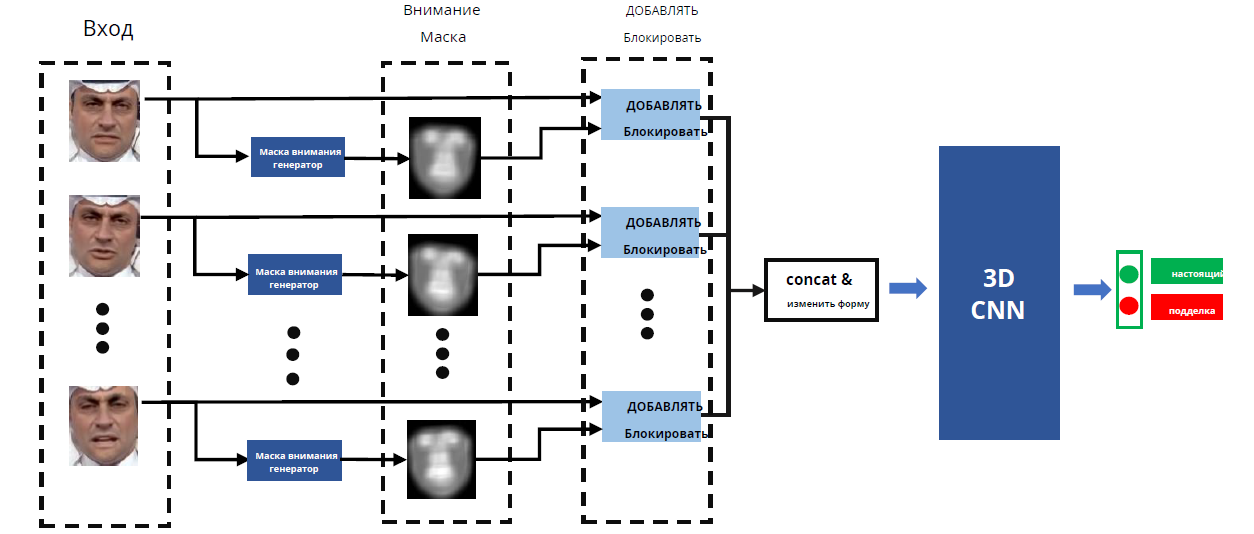
\includegraphics[width = 520 pt] {19.png}
            \caption{ADDNets 3D для обнаружения дипфейк подделок на уровне видеопоследовательностей}
        \end{figure}
        \newpage
    \subsection {Результаты обнаружения с помощью ADDNets}
        \begin{figure}[h!]
            \centering
            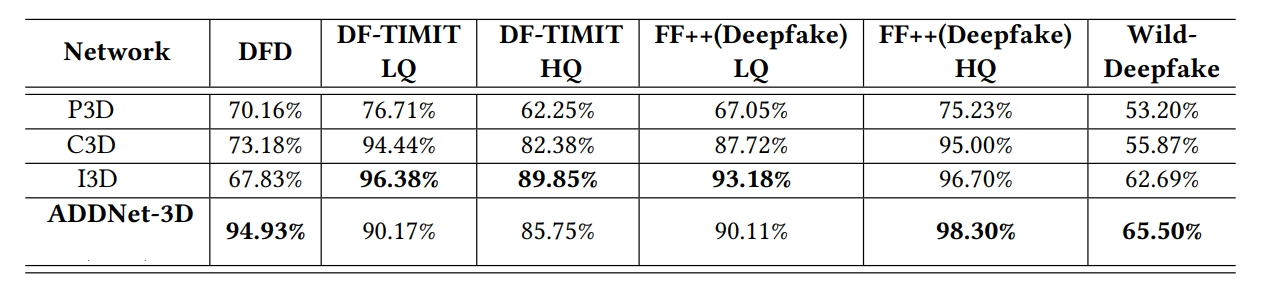
\includegraphics[width = 500 pt] {21.jpg}
            \caption{Сравнение уровня точности распознавания дипфейков с помощью ADDNet в зависимости от датасета}
        \end{figure}
        Рассматривались три существующих наборов данных DeepfakeDetection (DFD), DeepFake-Timit (DF-TIMIT) и FaceForensics++ (FF++), для последних двух было две версии , как низкое качество LQ, так и высокое качество HQ. , а также созданный датасет WildDeepfake. Точность обнаружения дипфейков – производительность метрики. Если с существующими наборами данных DFD, TIMIT, F++ точность распознавания доходит от 90 до 95\%, 
        то с дикими дипфейками никакие базовые сети не могу достичь точности выше 70\%.
        Среди базовых сетей I3D
обеспечивает лучшую производительность почти для всех протестированных
наборов данных, за исключением DFD, где C3D более эффективен. В частности,
I3D обеспечивает высокую точность обнаружения> 89\% для четырех наборов
данных DF-TIMIT и FF ++, тогда как C3D имеет точность 73,18\% для DFD. Опять же,
все они значительно падают на WildDeepfake с гораздо более низкой точностью
<63\%. Но ADDNet обеспечивает удивительно высокую точность 94,93\% на наборе DFD, не сильно отстает на наборах DF-TIMIT B FF++, но заметно лучше распознает WildDeepFake, чем остальные сети.\newline 
$\qquad$Исходя из [4] получаются разные результаты успеха верного вычисления дипфейков в зависимости от самих датасетов. И меньше всего точность распознавания у диких дипфейков, которые является более сложным набором данных, где производительность базовых детекторов может резко снизиться, т.к они состоят из лиц в движении, которых в кадре может быть несколько, а также изначально высокое качество видео.
        Также стоит отметить, что по сравнению с 2D-сетями обнаружения, 3D-сети, как правило, менее эффективны. Одной из возможных причин снижения производительности сетей трехмерного обнаружения является то, что временная информация, содержащаяся в последовательностях глубоких подделок лиц, также искажается из-за покадровой генерации поддельных лиц. Это указывает на то, что временная информация в дипфейке видео следует обрабатывать иначе, чем в реальном видео, чтобы повысить точность обнаружения глубоких подделок на уровне последовательности. 
    \newpage
    \section {Заключение}
        $\qquad$В данной работе были рассмотрены разные виды атак на видеопоследовательности и некоторые методы обнаружения этих атак.
        \begin{enumerate}
            \item Были исследованы атаки с пространственным вмешательством, временным вмешательством, пространственно-временным вмешательством и дипфейки.
            \item Были проанализированы активные и пассивные методы обнаружения, сеть обнаружения дипфейков на основе внимания ADDNets.
        \end{enumerate}
        \newline
        Необходимо продолжать исследовать атаки на видеопоследовательности и еще больше совершенствовать методы для их обнаружения.
    \newpage
    \begin{thebibliography}{9}
        \bibitem{latex:b1}
        S. Upadhyay, S.K. Singh. Video Authentication: Issues and Challenges, 2012.
        \bibitem{latex:b1}
        L.C.Manikandan, R. Habeeb. Video Tampering Attacks and Detection Techniques,2019
         \bibitem{latex:b1}
        S. Lyu. DeepFake Detection: Current Challenges and Next Steps, 2020.
        \bibitem{latex:b1}
        B. Zi, M. Chang, J. Chen, X. Ma, Y. Jiang. WildDeepfake: A Challenging Real-World Dataset for Deepfake Detection, 2021.
        \bibitem{latex:b1}
        N. Aggarwal, R.Singh. Video content authentication techniques: a comprehensive survey, 2017
        \bibitem{latex:b1}
        S. Upadhyay, S.K. Singh, M. Vatsa, and R. Singh. Video
        authentication using relative correlation information and SVM, 2008.
        \bibitem{latex:b1}
        A.Gandhi, S.Jain. Adversarial Perturbations Fool Deepfake Detectors, 2020.
        \bibitem{latex:b1}
        N. Ruiz, S.A. Bargal,S. Sclarof.Disrupting Deepfakes: Adversarial Attacks
Against Conditional Image Translation
Networks and Facial Manipulation Systems, 2020.
        \bibitem{latex:b1}
        P. Neekhara, B. Dolhansky, J. Bitton, C.C Ferrer. Adversarial Threats to DeepFake Detection: A Practical Perspective, 2020.
        \bibitem{latex:b1}
        P. Yin, H. Yu, Classification of Video Tampering: Methods and Countermeasures using Digital Watermarking, 2001
        \bibitem{latex:b1}
        Y.-J. Heo, Y.-J. Choi, Y.-W. Lee, B.-G. Kim. Deepfake Detection Scheme Based on Vision Transformer and Distillation, 2021.
        \bibitem{latex:b1}
        A. Gironi, M. Fontani, T. Bianchi, A. Piva, M. Barni. A video forensic technique for detecting frame deletion and insertion, 2014.
        \bibitem{latex:b1}
        Stamm, C. Matthew, W. Sabrina Lin, KJ Ray Liu. Temporal forensics and anti-forensics
for motion compensated video, 2012.
        \bibitem{latex:b1}
        N. Mondaini, R. Caldelli, A. Piva, M. Barni, and V.Cappellin. Detection of malevolent changes
in digital video for forensic applications, 2007.
        \bibitem{latex:b1}
        V. Amanipour, S. Ghaemmaghami. Video-Tampering Detection and Content Reconstruction via Self-Embedding, 2018.
        \bibitem{latex:b1}
        O.I. Al-Sanjary, G. Sulong. Detection of video forgery: a review of literature, 2015.
        \bibitem{latex:b1}
        J. Hussein, A. Mohammed. Robust Video Watermarking using Multi-Band
Wavelet Transform, 2009.
        \bibitem{latex:b1}
        R. Tolosana, R. Vera-Rodriguez, J. Fierrez, A. Morales, J. Ortega-Garcia. DeepFakes and Beyond: A Survey of Face Manipulation and Fake Detection, 2020.
        \bibitem{latex:b1}
        B. Dolhansky, J. Bitton, B. Pflaum, J. Lu, R. Howes, M. Wang, C. C. Ferrer. The DeepFake Detection Challenge (DFDC) Dataset.
        \bibitem{latex:b1}
        S. Fung, X. Lu, C. Zhang, C.-T. Li. DeepfakeUCL: Deepfake Detection via
Unsupervised Contrastive Learning, 2021.
        
    \end{thebibliography}





        


\end{document}
